\documentclass{wscpaperproc}
% \usepackage[spanish, activeacute]{babel}
\usepackage{latexsym}
%\usepackage{caption}
\usepackage{graphicx}
\usepackage{mathptmx}
\usepackage[T1]{fontenc}
\usepackage{amsmath}
\usepackage{setspace}

%
%****************************************************************************
% AUTHOR: You may want to use some of these packages. (Optional)
\usepackage{amsmath}
\usepackage{amsfonts}
\usepackage{amssymb}
\usepackage{amsbsy}
\usepackage{amsthm}
%****************************************************************************


%
%****************************************************************************
% AUTHOR: If you do not wish to use hyperlinks, then just comment
% out the hyperref usepackage commands below.

%% This version of the command is used if you use pdflatex. In this case you
%% cannot use ps or eps files for graphics, but pdf, jpeg, png etc are fine.

\usepackage[colorlinks=true,urlcolor=blue,citecolor=black,anchorcolor=black,linkcolor=red]{hyperref}
%\usepackage{hyperref}

%% The next versions of the hyperref command are used if you adopt the
%% outdated latex-dvips-ps2pdf route in generating your pdf file. In
%% this case you can use ps or eps files for graphics, but not pdf, jpeg, png etc.
%% However, the final pdf file should embed all fonts required which means that you have to use file
%% formats which can embed fonts. Please note that the final PDF file will not be generated on your computer!
%% If you are using WinEdt or PCTeX, then use the following. If you are using
%% Y&Y TeX then replace "dvips" with "dvipsone"

%%\usepackage[dvips,colorlinks=true,urlcolor=blue,citecolor=black,%
%% anchorcolor=black,linkcolor=black]{hyperref}
%****************************************************************************


%
%****************************************************************************
%*
%* AUTHOR: YOUR CALL!  Document-specific macros can come here.
%*
%****************************************************************************

% If you use theoremes
\newtheoremstyle{wsc}% hnamei
{3pt}% hSpace abovei
{3pt}% hSpace belowi
{}% hBody fonti
{}% hIndent amounti1
{\bf}% hTheorem head fontbf
{}% hPunctuation after theorem headi
{.5em}% hSpace after theorem headi2
{}% hTheorem head spec (can be left empty, meaning `normal')i

\theoremstyle{wsc}
\newtheorem{theorem}{Teorema}
\renewcommand{\thetheorem}{\arabic{theorem}}
\newtheorem{corollary}[theorem]{Corolario}
\renewcommand{\thecorollary}{\arabic{corollary}}
\newtheorem{definition}{Definición}
\renewcommand{\thedefinition}{\arabic{definition}}


%#########################################################
%*
%*  The Document.
%*
\begin{document}

%***************************************************************************
% AUTHOR: AUTHOR NAMES GO HERE
% FORMAT AUTHORS NAMES Like: Author1, Author2 and Author3 (last names)
%
%		You need to change the author listing below!
%               Please list ALL authors using last name only, separate by a comma except
%               for the last author, separate with "and"
%
\WSCpagesetup{Álvarez, Cordero, Díaz, Guerra, and Llerena}
% \pagestyle{myheadings}
% \markright{Álvarez, Cordero, Díaz, Guerra, and Llerena}

% AUTHOR: Enter the title, all letters in upper case
\title{Análisis de {\it Stability and Numerical Simulation of Prey-predator System with Holling
			Type-II Functional Responses for Adult Prey} [1]}

% AUTHOR: Enter the authors of the article, see end of the example document for further examples
\author{
	Pedro Pablo Álvarez Portelles\\[12pt]
	Grupo C212\\
	Ciencia de la Computación\\
	Facultad de Matemática y Computación\\
	Universidad de La Habana. Cuba\\
	% Multiple authors are entered as follows.
	% You may also need to adjust the titlevbox size in the preamble - search for titlevboxsize
	\and
	Amanda Cordero Lezcano\\[12pt]
	Grupo C212\\
	Ciencia de la Computación\\
	Facultad de Matemática y Computación\\
	Universidad de La Habana. Cuba\\
	\and
	Marlon Díaz Pérez\\[12pt]
	Grupo C212\\
	Ciencia de la Computación\\
	Facultad de Matemática y Computación\\
	Universidad de La Habana. Cuba\\
	\and
	Christopher Guerra Herrero\\[12pt]
	Grupo C212\\
	Ciencia de la Computación\\
	Facultad de Matemática y Computación\\
	Universidad de La Habana. Cuba\\
	\and
	Abel Llerena Domínguez\\[12pt]
	Grupo C212\\
	Ciencia de la Computación\\
	Facultad de Matemática y Computación\\
	Universidad de La Habana. Cuba\\
}



\maketitle

\section*{Resumen}
Este artículo constituye un análisis de [1], el cual examina la estabilidad de un modelo de presa-depredador.
Se analizan los puntos de equilibrio y se realiza una exploración numérica
para mostrar los resultados. Estos confirman los hallazgos analíticos
y revelan el comportamiento del modelo, considerando las interacciones entre presas
jóvenes, adultas y depredadores.
\section{INTRODUCCIóN}
\label{sec:intro}
El propósito de este documento es hacer un análisis de [1], artículo elaborado por la especialista analítica Dian Savitri. Fue presentado en el MISEIC(Matematics,
Informatics, Science and Education International Conference) en 2019 y publicado en Journal of Physics: Conference Series, bajo la licencia de IOP Publishing.
Factor de impacto del artículo: 0.227, en la fecha de publicación del artículo. Actualmente la revista tiene un factor de impacto de 0.21.

	{\bf Valoración del artículo:} Los autores consideramos que [1] presenta varios errores, tanto tipográfico como de contenidos. Su factor de impacto es
relativamente bajo. Sin embargo consideramos que se tratan temáticas muy interesantes y de gran utilidad para el desarrollo de la ecología.

{\bf Objetivo del artículo:} Analizar la estabilidad de un modelo presa-depredador.


El modelo fue construido a partir de dos presas que involucran una estructura de etapa y un depredador. Posee tres equilibrios positivos: el original, la extinción del
depredador y un punto interior. El artículo hace un estudio de la dinámica
del comportamiento de las interacciones presa-depredador, con la función de respuesta Holling tipo II(esta respuesta funcional se
refiere al cambio en el comportamiento de los individuos en función de la densidad del huésped o presa) para presas adultas. El apartado considera la estabilidad de
los equilibrios en detalle con las condiciones de existencia e ilustra la estabilidad local de los equilibrios, además cuenta con simulaciones numéricas para ilustrar
los resultados.

\subsection*{Técnicas utilizadas:}
\begin{itemize}
	\item Criterio Routh Hurwitz: consiste en un simple procedimiento o algoritmo para poder determinar si existe alguna raíz o polo en el semiplano derecho del
	      plano complejo “s”, donde si al menos existe una raíz el sistema es inestable, caso contrario si no hay ninguna raíz en el semiplano derecho el sistema es estable.
	\item Usando python y una implementación computacional del método Runge-Kutta de orden 4 se resolvió el sistema presa-depredador.
\end{itemize}
\subsection{Estructura del trabajo}
\begin{itemize}
	\item Modelo matemático
	\item Análisis de los puntos de equilibrio
	\item Simulaciones numéricas
\end{itemize}

\section{Resultados fundamentales.}


Ecuaciones que ilustran el modelo matemático utilizado:

\begin{eqnarray}\label{dx}
	\frac{dx}{dt} &=& rx(1-\frac{x}{k})-\beta x-\alpha xz
\end{eqnarray}
\begin{eqnarray}\label{dy}
	\frac{dy}{dt} &=& \beta x-\frac{\eta yz}{y+m}-\mu y
\end{eqnarray}
\begin{eqnarray}\label{dz}
	\frac{dz}{dt} &=& \alpha_1 xz+\rho z^2-\frac{\eta_1z^2}{y+m}
\end{eqnarray}



\vspace*{1cm}

{\bf Ecuación \ref*{dx}}
\begin{itemize}
	\item El término $rx(1-\frac{x}{k})$ de (\ref*{dx}) es conocido como ecuación
	      logística y se compone por:
	      \vspace*{0.3cm}

	      $x$: población de presas juveniles.

	      $t$: tiempo.

	      $r$: constante que define la tasa de crecimiento.

	      $k$: capacidad de carga o persistencia.

	      \vspace*{0.5cm}

	      Esta primera ecuación representa el modelo de crecimiento poblacional en las
	      presas jóvenes. Para ello se tuvo en cuenta:
	      \begin{itemize}
		      \item La tasa de reproducción es proporcional a la población existente.
		      \item La tasa de reproducción es proporcional a la cantidad de recursos disponibles.
		      \item La competición por los recursos disponibles tiende a limitar el crecimiento poblacional.
	      \end{itemize}

	\item $\beta x$ representa las presas que se vuelven adultas.

	      \vspace*{0.3cm}

	      $\beta$: factor de conversión de presa joven a presa adulta

	      \vspace*{0.3cm}

	\item La velocidad con que varía la población de presas $x$ es proporcional al número de encuentros con los depredadores $z$ según la ecuación de Lotka-Volterra:
	      $$\frac{dx}{dt}=\alpha xz$$
	      $\alpha$: tasa de eliminación de presas por parte de los depredadores.
\end{itemize}

\vspace*{1cm}
{\bf Ecuación \ref*{dy}}
Por otra parte (\ref*{dy}) se refiere a la población de presas adultas.

\begin{itemize}
	\item El primer término de la ecuación ya fue analizado anteriormente, es la cantidad de presas jóvenes que se convierten en adultas.

	\item El proceso de eliminación de presas por los depredadores se describe a partir del modelo Holling Tipo II, que establece:

	      $$\frac{dy}{dt} = -\frac{\eta yz}{y+m}$$

	      donde:

	      $\eta$: valor máximo de la tasa de reducción per cápita de presas adultas debido a los depredadores.

	      $m$: coeficiente de protección ambiental para las presas adultas.

	\item Además se considera las presas que mueren de forma natural $\mu y$.

	      $\mu$: tasa de mortalidad en presas adultas.
\end{itemize}

\vspace*{1cm}
{\bf Ecuación \ref*{dz}}
Por último (\ref*{dz}) modela la población de depredadores.

\begin{itemize}
	\item $\alpha_1 xz$ responde al modelo de Lotka-Volterra. Esta ecuación representa que el crecimiento de los depredadores es
	      proporcional a la caza de presas juveniles.

	      $\alpha_1$: tasa de crecimiento de los depredadores debido a la caza de presas juveniles.

	      \vspace*{0.3cm}

	\item $\rho z^2$ es el crecimiento intrínseco.

	      $\rho$: tasa de crecimiento intrínseco.

	\item El tercer término representa la tasa de mortalidad en el esquema de Leslie Gower.

	      $\eta_1$: relación del crecimiento intríseco y el factor de conversión de depredación a presa adulta.

	      $m$: pérdida residual de los depredadores.

	      Esta consideración está basada en la idea de una relación entre la reducción de la población de depredadores y la
	      disponibilidad per cápita de sus comida favorita. Esta disponibilidad está condicionada por la abundancia de alimentos
		  y las características medioambientales.
\end{itemize}
\vspace*{3cm}
{\it En \ref*{dz} discrepamos de [1]. Consideramos que Savitri pudo tener un error tipográfico, pues en lo adelante asume nuestra
ecuación, además [2] defiende este modelo.}

\section*{Análisis de los puntos de equilibrio y su estabilidad}

Los puntos de equilibrio para este sistema son aquellos que satisfacen:
$$\frac{dx}{dt}=\frac{dy}{dt}=\frac{dz}{dt}=0$$

Estos puntos son:
\begin{itemize}
	\item $P_1=(0, 0, 0)$
	\item $P_2=(\frac{k(r-\beta)}{r}, \frac{\beta k(r-\beta)}{\mu r}, 0)$
	\item $P_3=(x_3, y_3, z_3)$
\end{itemize}

La estabilidad de los puntos de equilibrio se puede analizar calculanfo la matriz Jacobiana. Para nuestro sistema sería:
$$ J(x^*, y^*, z^*) = \left(
	\begin{array}{ccc}
			r-\frac{2rx}{k}-\beta-\alpha z & 0                                       & -\alpha x                       \\
			\beta                          & \frac{-nz}{y+m}+\frac{nyz}{(y+m)^2}-\mu & \frac{-ny}{y+m}                 \\
			\alpha_1z                      & \frac{n_1z^2}{(y+m)^2}                  & 2pz-\frac{2n_1z}{y+m}+\alpha_1x
		\end{array}
	\right)$$

La ecuación característica esta dada por el $det(J(x^*, y^*, z^*)-I)=0$ donde $(x^*, y^*, z^*)$ es un punto de equilibrio del sistema.
Nosotros solo analizaremos la estabilidad de los puntos de equilibrio no negativos por la parte real de los valores propios de la matriz Jacobiana.
\vspace*{0.5cm}
Para $P_1$ sería:
$$\left|
	\begin{array}{ccc}
		(-\beta+r)-\lambda & 0            & 0        \\
		\beta              & -\mu-\lambda & 0        \\
		0                  & 0            & -\lambda
	\end{array}
	\right| =0$$

{\it En este punto, [1] se refiere a $-1+r$ donde nosotros a $-\beta+r$. Consideramos que haya sido un error tipográfico, pues como bien ella
		afirma, esta matriz se obtiene al sustituir el punto de equilibrio (0, 0, 0).}


De ahí que sus valores propios están dados por $((-\beta+r)-\lambda)(-\mu-\lambda)(-\lambda)=0$. Pero esta ecuación siempre tiene valor negativo
\textcolor{red}{$\lambda_1=-$}, también si $r<\beta$, pero \textcolor{red}{$\lambda_3=0$}. Por tanto en $P_1$ el sistema es inestable.

\vspace*{0.5cm}

Para $P_2$ sería:
$$\left|
	\begin{array}{ccc}
		(\beta+r)-\lambda & 0            & \frac{\alpha k(\beta-r)}{r}                                      \\
		\beta             & -\mu-\lambda & \frac{n\beta k(\beta-r)}{r\mu (\frac{\beta k(r-\beta)}{r\mu}+m)} \\
		0                 & 0            & \frac{\alpha_1 k(\beta-r)}{r}-\lambda
	\end{array}
	\right| =0$$

{\it En la tercera fila, tercera columna, [1] olvida restar $\lambda$, asumimos error tipográfico}

Que luego de un poco de trabajo algebraico obtendrías $\textcolor{red}{\lambda_1=\beta-r, \lambda_2=cosa q no entiendo, \lambda_3=\frac{\alpha_1 k(\beta-r)}{r}}$. Por lo que $P_2$ es inestable.

	{\it [1] considera este punto estable, diferimos de su resultado}


\vspace*{0.5cm}

En el caso $P_3$ sería:
$$ J(x_3, y_3, z_3) = \left(
	\begin{array}{ccc}
			r-\frac{2rx_3}{k}-\beta-\alpha z_3 & 0                                                 & -\alpha x_3                             \\
			\beta                              & \frac{-nz_3}{y_3+m}+\frac{ny_3z_3}{(y_3+m)^2}-\mu & \frac{-ny_3}{y_3+m}                     \\
			\alpha_1z_3                        & \frac{n_1z_3^2}{(y_3+m)^2}                        & 2pz_3-\frac{2n_1z_3}{y_3+m}+\alpha_1x_3
		\end{array}
	\right)$$

La ecuación característica entonces es de la forma:
$$\lambda^3+\gamma_1\lambda^2+\gamma_2\lambda+\gamma_3=0 $$

{\it Aquí [1] trabaja con $\lambda^2-\ traza\ \lambda+\ deteminante$, esto no es aplicable para sistemas mayores que dos, ni
es resultado de simplificación alguna}

Si usamos el criterio Routh-Hurwitz para analizar la estabilidad en $P_3$ veremos que este
tiene una parte real negativa si y solo si $\gamma_1>0, \gamma_3>0$ y $\gamma_1\gamma_2-\gamma_3>0$, la coexistencia en $P_3$ es local
y asintóticamente estable.

\vspace*{3cm}


\section*{Métodos y algoritmos utilizados}


\subsection*{Ejemplos Numéricos. Reproducción de los experimentos}

Para reproducir los experimentos se utilizó el método de Runge-Kutta de orden 4 (RK4), programado
en Python 3.10 y haciendo uso de librerías para la manipulación eficiente de vectores como Numpy y
Scipy.

El metodo de Runge-Kutta es método de un paso en el cual se usa un tamaño de paso $h$ para calcular
los siguientes valores a partir de valores previos.

Como en este trabajo se utiliza un sistema de tres ecuaciones,
es necesario de manera análoga crear otras variables $l$ y $m$ para
las funciones $y$ y $z$. El pseudocódigo sería de la siguiente manera:


\doublespacing
\begin{equation*}
	\begin{split}
		for\ i=0\ to\ n - 1:\\
		&xn = x[i];yn = y[i];zn = z[i]\\
		\\
		&k_1 = f_1(t_n, x_n, y_n, z_n)\\
		&l_1 = f_2(t_n, x_n, y_n, z_n)\\
		&m_1 = f_3(t_n, x_n, y_n, z_n)\\
		&k_2 = f_1(t_n + \frac{h}{2}, x_n + \frac{k_1}{2}, y_n + \frac{l_1}{2}, z_n + \frac{m_1}{2})\\
		&l_2 = f_2(t_n + \frac{h}{2}, x_n + \frac{k_1}{2}, y_n + \frac{l_1}{2}, z_n + \frac{m_1}{2})\\
		&m_2 = f_3(t_n + \frac{h}{2}, x_n + \frac{k_1}{2}, y_n + \frac{l_1}{2}, z_n + \frac{m_1}{2})\\
		&k_3 = f_1(t_n + \frac{h}{2}, x_n + \frac{k_2}{2}, y_n + \frac{l_2}{2}, z_n + \frac{m_2}{2})\\
		&l_3 = f_2(t_n + \frac{h}{2}, x_n + \frac{k_2}{2}, y_n + \frac{l_2}{2}, z_n + \frac{m_2}{2})\\
		&m_3 = f_3(t_n + \frac{h}{2}, x_n + \frac{k_2}{2}, y_n + \frac{l_2}{2}, z_n + \frac{m_2}{2})\\
		&k_4 = f_1(t_n + h, x_n + k_3, y_n + l_3, z_n + m_3)\\
		&l_4 = f_2(t_n + h, x_n + k_3, y_n + l_3, z_n + m_3)\\
		&m_4 = f_3(t_n + h, x_n + k_3, y_n + l_3, z_n + m_3)\\
		\\
		&t[i+1] = t[i] + h\\
		&x[i+1] = \frac{h}{6}(k_1 + \frac{k_2}{2} + \frac{k_3}{3} + k_4)\\
		&y[i+1] = \frac{h}{6}(l_1 + \frac{l_2}{2} + \frac{l_3}{3} + l_4)\\
		&z[i+1] = \frac{h}{6}(m_1 + \frac{m_2}{2} + \frac{m_3}{3} + m_4)\\
	\end{split}
\end{equation*}
\singlespacing

El tamaño de paso se estableció para todos los experimentos en
$h=2^{-10}$ con el cual se obtienen resultados muy exactos teniendo
en cuenta que el error de RK4 es del orden $O(h^5)$, con lo que tendriamos
que el error sería aproximadamente del orden de $e \approx 2^{-50}$.

\subsection*{Reproducción de los experimentos}

Para los experimentos se utilizaron para los parámetros los valores de la siguiente tabla:

\begin{tabular}{p{1cm} | p{1cm} | p{1cm} | p{1cm} | p{1cm} | p{1cm} | p{1cm} | p{1cm} | p{1cm} }
	% aslask & gahbh
	$\#$ & $r$  & $\alpha$ & $\alpha_1$ & $\eta$ & $\eta_1$ & $K$  & $\rho$ & $m$  \\
	1    & 0.82 & 1.56     & 1.12       & 2.41   & 1.83     & 12.0 & 1.38   & 0.13 \\
	2    & 1.32 & 1.56     & 0.72       & 2.41   & 0.41     & 2.8  & 1.38   & 0.23 \\
	3    & 1.32 & 0.76     & 0.72       & 0.6    & 0.41     & 2.8  & 0.78   & 0.23 \\
	4    & 0.82 & 0.76     & 0.72       & 1.2    & 0.41     & 2.8  & 1.38   & 0.23 \\
	5    & 1.32 & 1.16     & 0.72       & 0.31   & 0.41     & 2.8  & 0.78   & 0.23 \\
\end{tabular}
\\

Además, se usó fijo $\beta=0.87$ y $\mu=0.11$.

	{\it note que [1] da dos interpretaciones diferentes para la variable $m$, sin embargo ambos conceptos se simulan con igual magnitud}

\vspace*{0.5cm}
{\bf Primer experimento}

En el primer conjunto de experimentos se usaron los valores iniciales $[x_0=3.01, y_0=5.05, z_0=4.28]$ (1.1)
y $[x_0=4.6, y_0=5.9, z_0=3.1]$(1.2).

\begin{figure}[h!]
	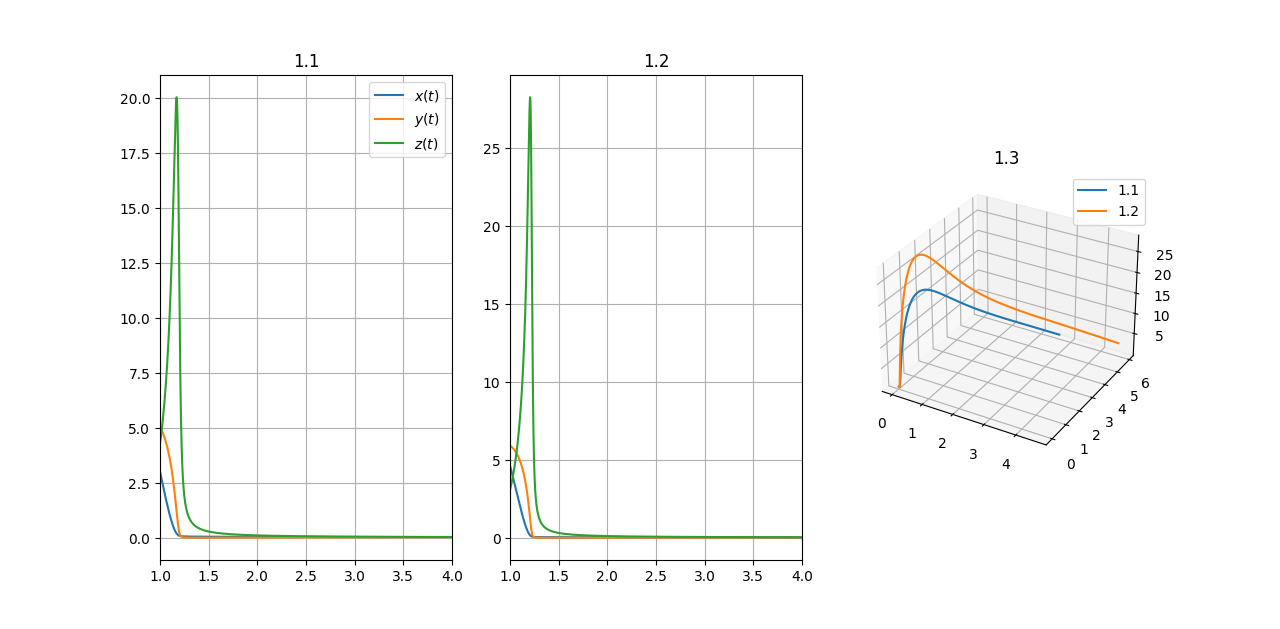
\includegraphics[width=\linewidth]{../numerical_models/images/1.png}
	\caption{Experimento \#1}
\end{figure}

\vspace*{7cm}
{\bf Segundo experimento}

En el segundo conjunto de experimentos, se usaron valores tal que $\eta > \beta$ y $\eta > \alpha$.
De valores iniciales se utilizaron $[x_0=0.3, y_0=2.4, z_0=3.9]$(2.1),
$[x_0=0.6, y_0=2.4, z_0=3.9]$(2.2) y $[x_0=2.1, y_0=1.2, z_0=1.1]$

La simulación muestra que todos los valores van al punto de equilibrio interior.

\begin{figure}[h!]
	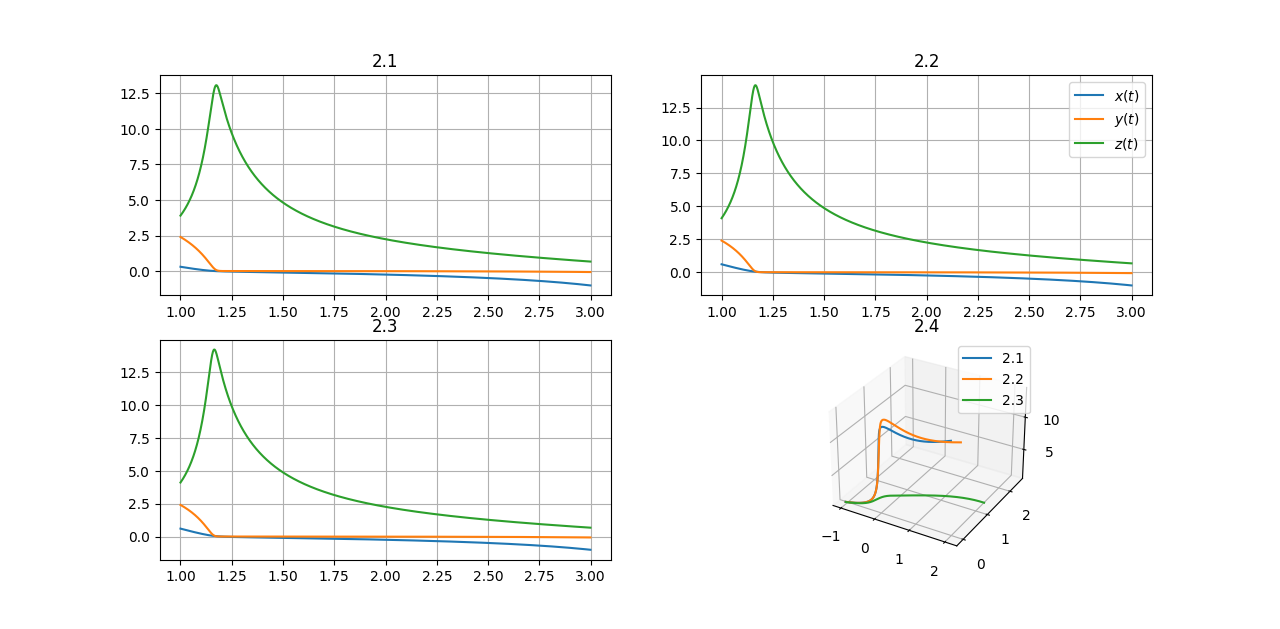
\includegraphics[width=\linewidth]{../numerical_models/images/2.png}
	\caption{Experimento \#2}
\end{figure}

\vspace*{4cm}
{\bf Tercer experimento}

En el tercer experimento, se usaron valores tal que $\alpha > \beta$
Los valores iniciales usados fueron $[x_0=0.3, y_0=2.4, z_0=3.9]$. La simulación muestra
que los valores van al punto de equilibrio.

	{\it Este experimento difiere del resultado dado por [1]}

\begin{figure}[h!]
	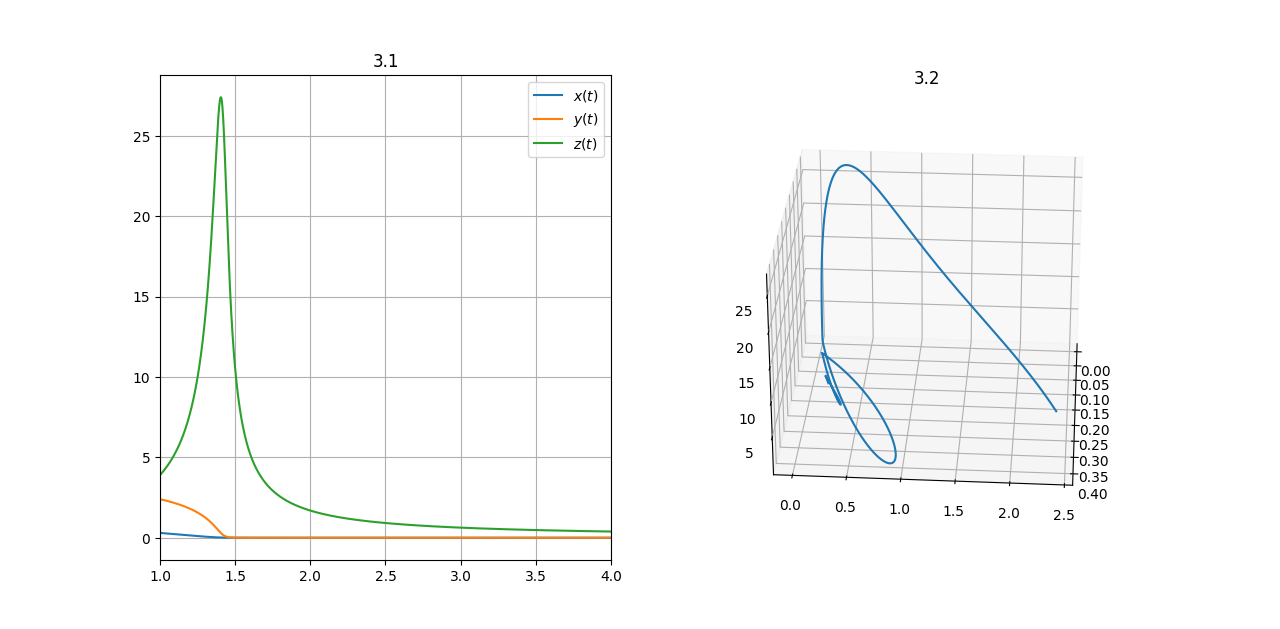
\includegraphics[width=\linewidth]{../numerical_models/images/3.png}
	\caption{Experimento \#3}
\end{figure}

\vspace*{7cm}
{\bf Cuarto experimento}

En el cuarto experimento, se usaron valores tal que $\eta = \alpha$.
Los valores iniciales usados fueron $[x_0=1.2, y_0=2.1, z_0=4.28]$. La simulación muestra
que los valores van al punto de equilibrio.

\begin{figure}[h!]
	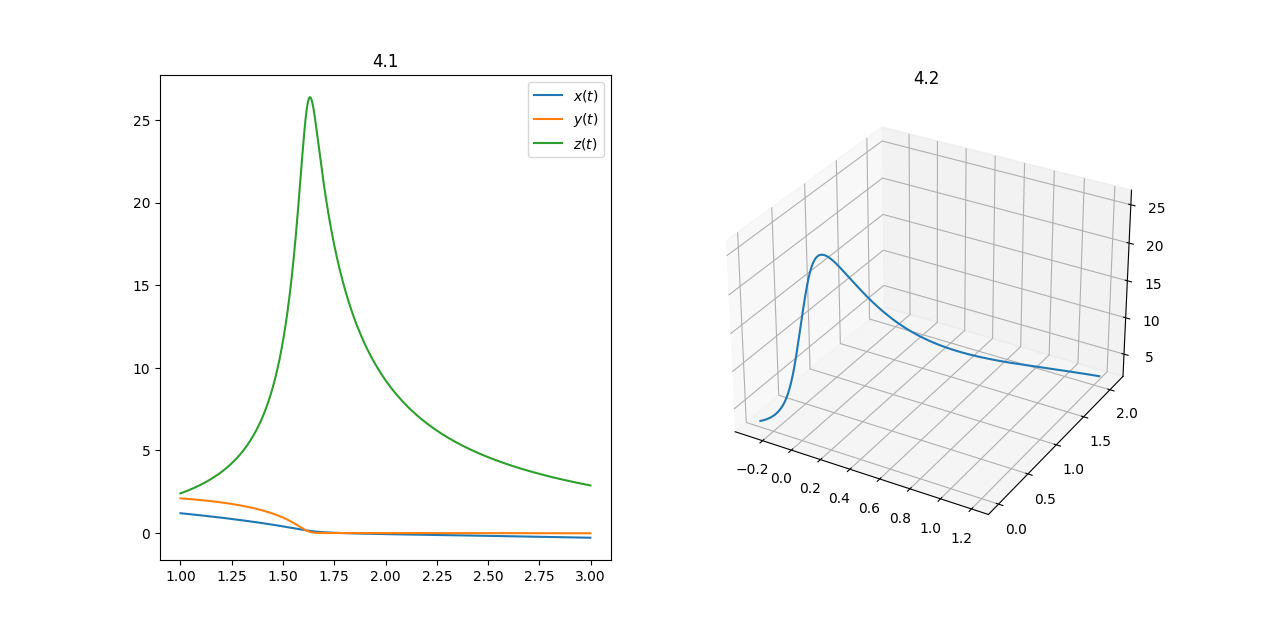
\includegraphics[width=\linewidth]{../numerical_models/images/4.png}
	\caption{Experimento \#4}
\end{figure}

\vspace*{7cm}
{\bf Quinto experimento}

En el quinto experimento, se usaron valores tal que $\eta > \beta$ y $\eta > \alpha$.
Los valores iniciales usados fueron $[x_0=1.2, y_0=2.1, z_0=2.4]$. La simulación muestra
que los valores van al punto de equilibrio.

\begin{figure}[h!]
	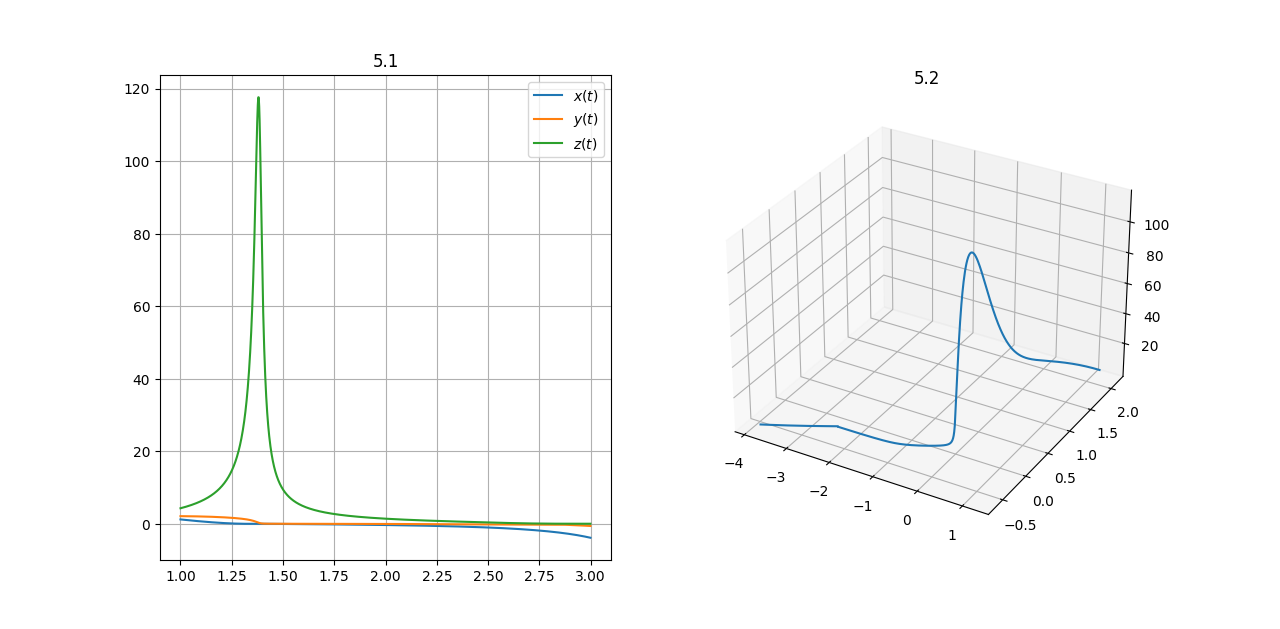
\includegraphics[width=\linewidth]{../numerical_models/images/5.png}
	\caption{Experimento \#5}
\end{figure}

\vspace*{4cm}




\section*{Conclusiones}

Este estudio ha examinado la estabilidad de un modelo de interacción presa-depredador con estructura
de etapas en las poblaciones de presas. Se han identificado y analizado los puntos de equilibrio,
encontrando tres equilibrios positivos: el inicial, la extinción del depredador y el punto interior.
Se ha demostrado que el punto interior es localmente estable bajo ciertas condiciones. Las simulaciones
numéricas han respaldado los resultados analíticos, proporcionando evidencia adicional del comportamiento
del modelo. Estos hallazgos contribuyen a mejorar nuestra comprensión de los sistemas ecológicos. Esta línea de trabajo
podría continuar estudiando los términos que componen el modelo para lograr un mayor ajuste a la realidad de la
naturaleza.


\vspace*{3cm}

{\bf \Large Referencias}

\ [1]\ {D. Savitri, Stability and Numerical Simulation of Prey-predator System with Holling
Type-II Functional Responses for Adult Prey}.

\ [2]\ {L. Gauer esa}


\end{document}

